\chapter{Preliminary Work}
\label{chapter:preliminary}

This chapter presents the work carried out during the first phase of the
project, covering hardware assembly, firmware development, initial validation
experiments, and preliminary data collection.
The prototype is fully functional and the results described here demonstrate
the viability of the proposed sensing approach as a basis for the planned
data acquisition campaigns.

% ----------------------------------------------------------------------
\section{Hardware Prototype}
\label{section:hw_prototype}

A working prototype of the instrumented prosthesis has been assembled and
validated.
The system integrates all sensing, processing, and storage components in a
compact embedded platform designed to fit within the structural constraints
of the prosthetic device.

Figure~\ref{fig:prototype_exterior} shows the exterior of the assembled
prosthesis, and Figure~\ref{fig:prototype_interior} shows the internal
electronics.
Table~\ref{tab:hw_components} lists the main components and their roles.
The MPU-9250 and microSD card share the SPI bus with independent chip-select
lines; the HX711 uses a dedicated two-wire interface.
Two 250\,mAh LiPo cells connected in parallel supply 500\,mAh at 3.7\,V
to the microcontroller's onboard 3.3\,V regulator.
Battery voltage is monitored continuously via an analog pin.

\begin{figure}[ht]
  \centering
  \begin{minipage}[t]{0.46\textwidth}
    \centering
    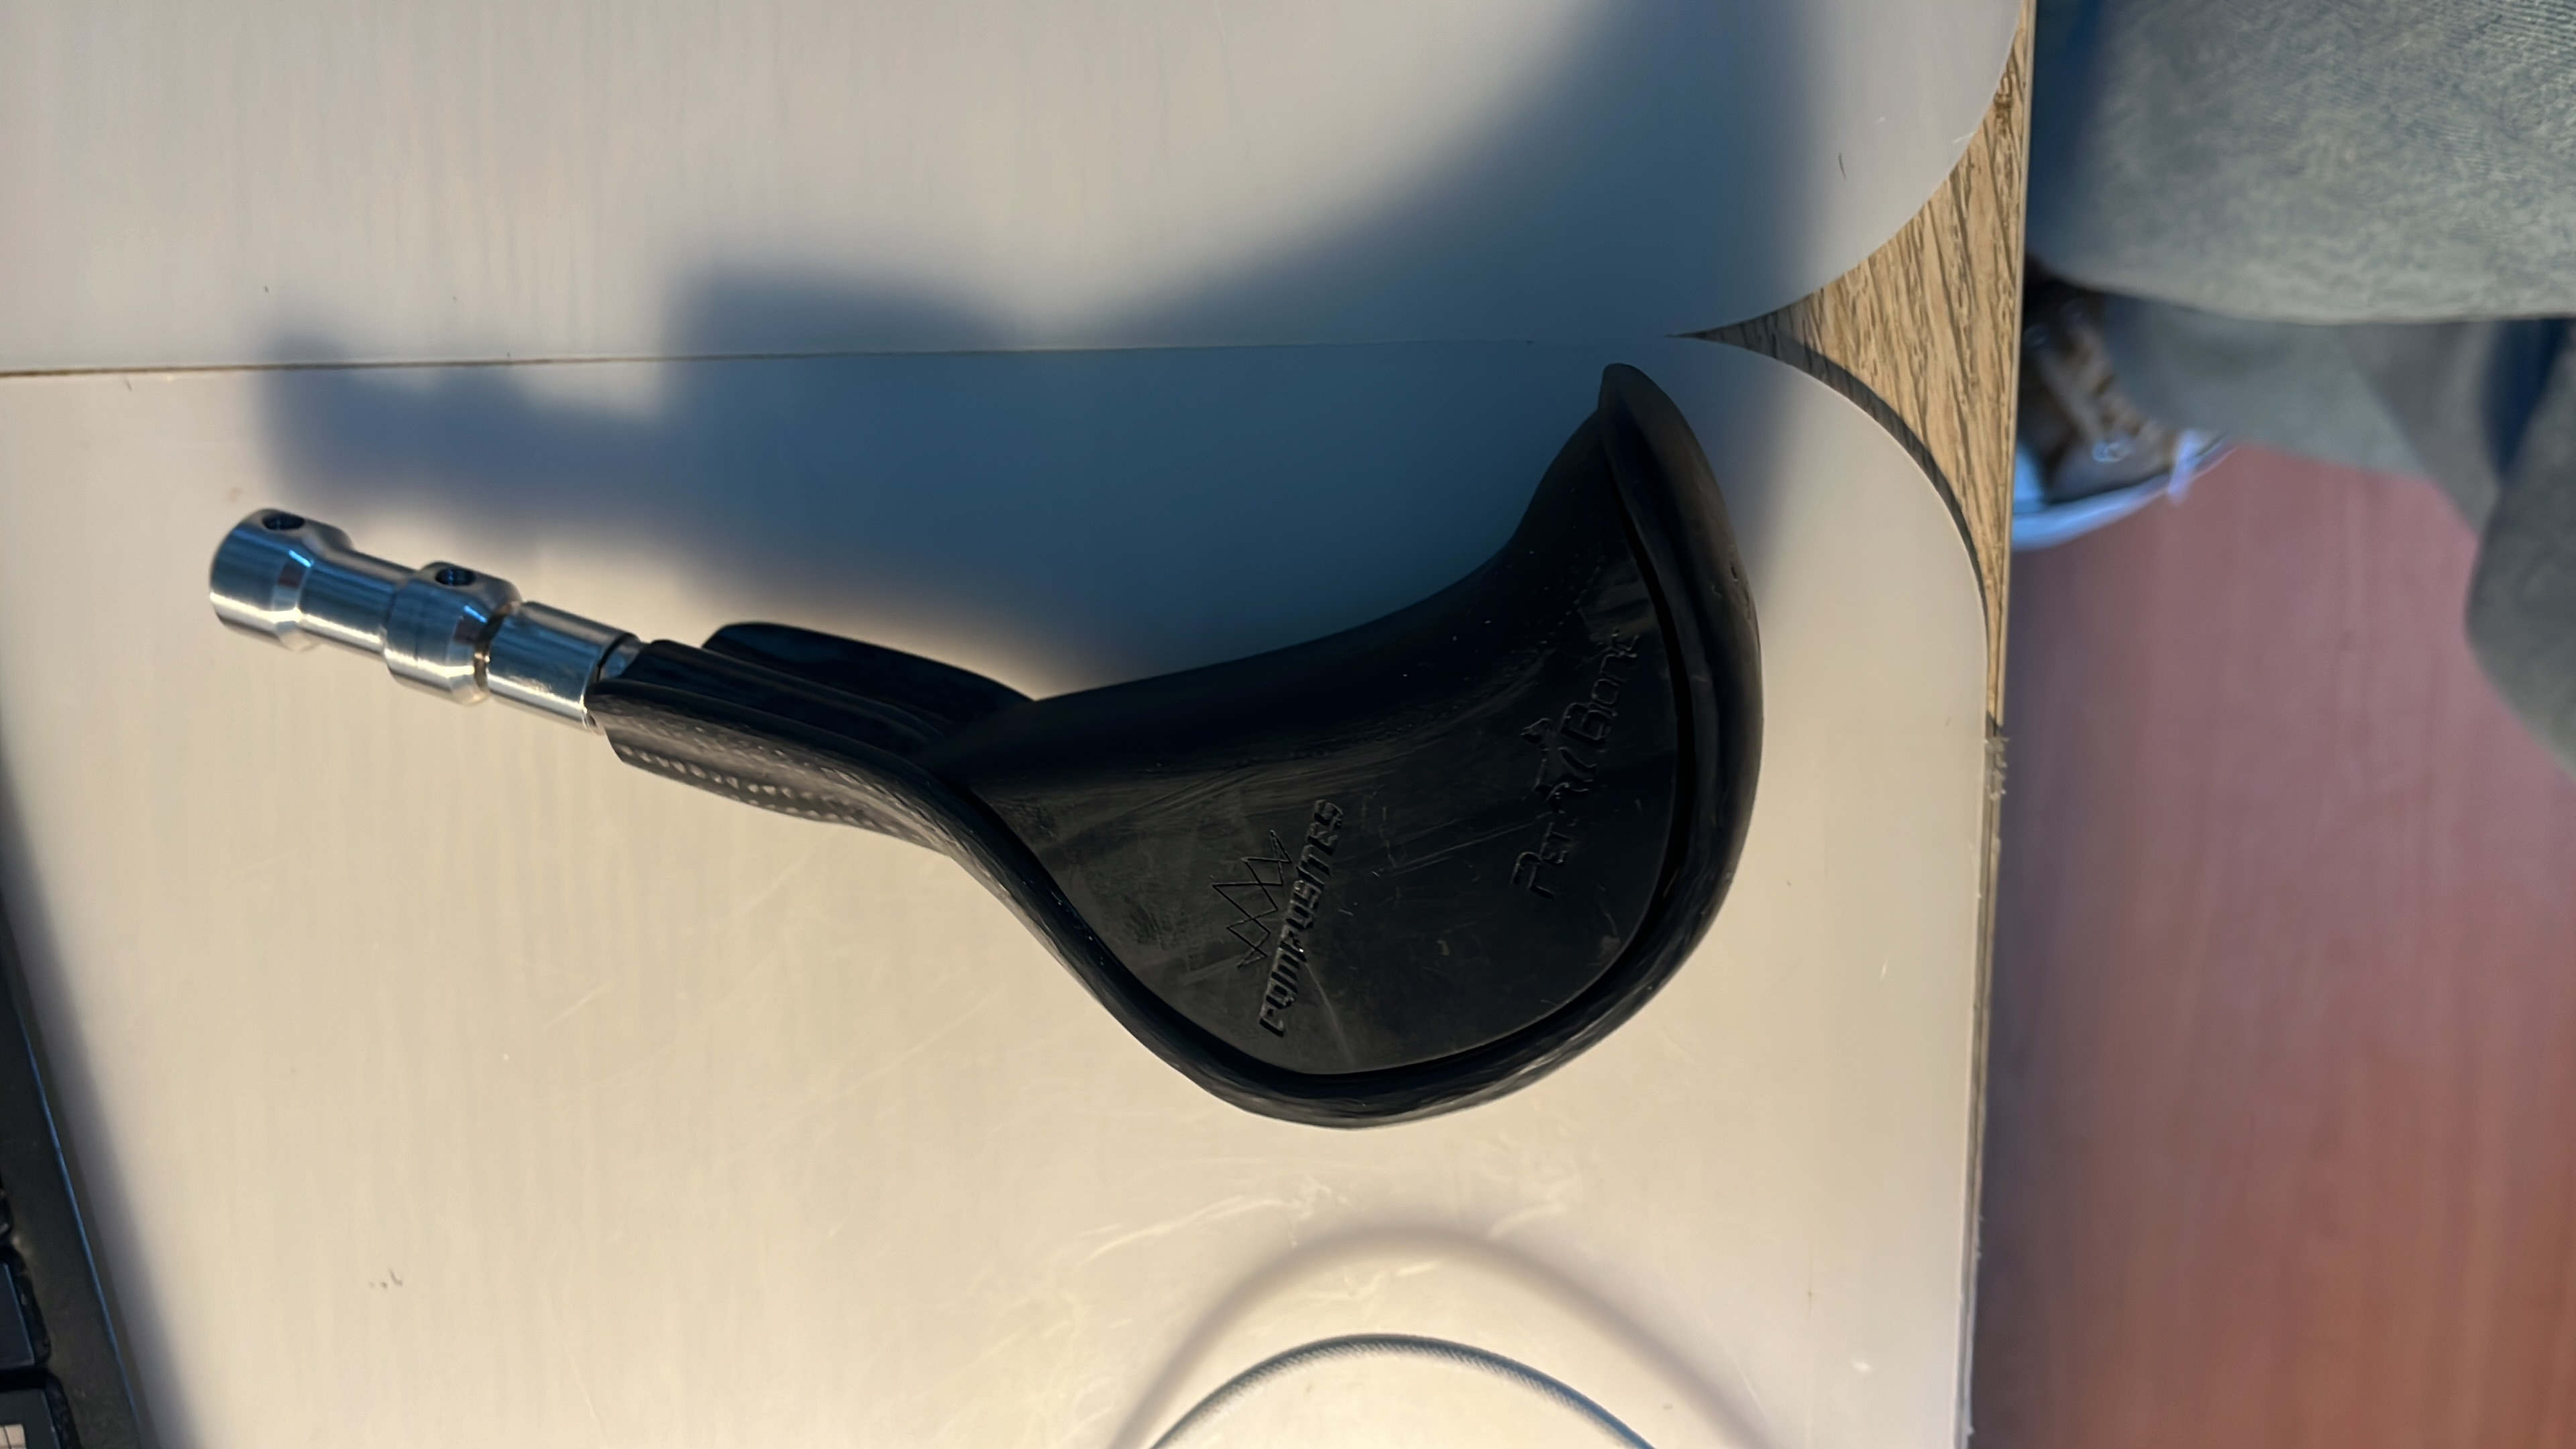
\includegraphics[width=\linewidth]{05_figures/06_preliminary/prototype_exterior}
    \caption{Assembled instrumented prosthesis — exterior view. The USB-C
             charging port and PetBionic branding are visible on the housing.}
    \label{fig:prototype_exterior}
  \end{minipage}
  \hfill
  \begin{minipage}[t]{0.50\textwidth}
    \centering
    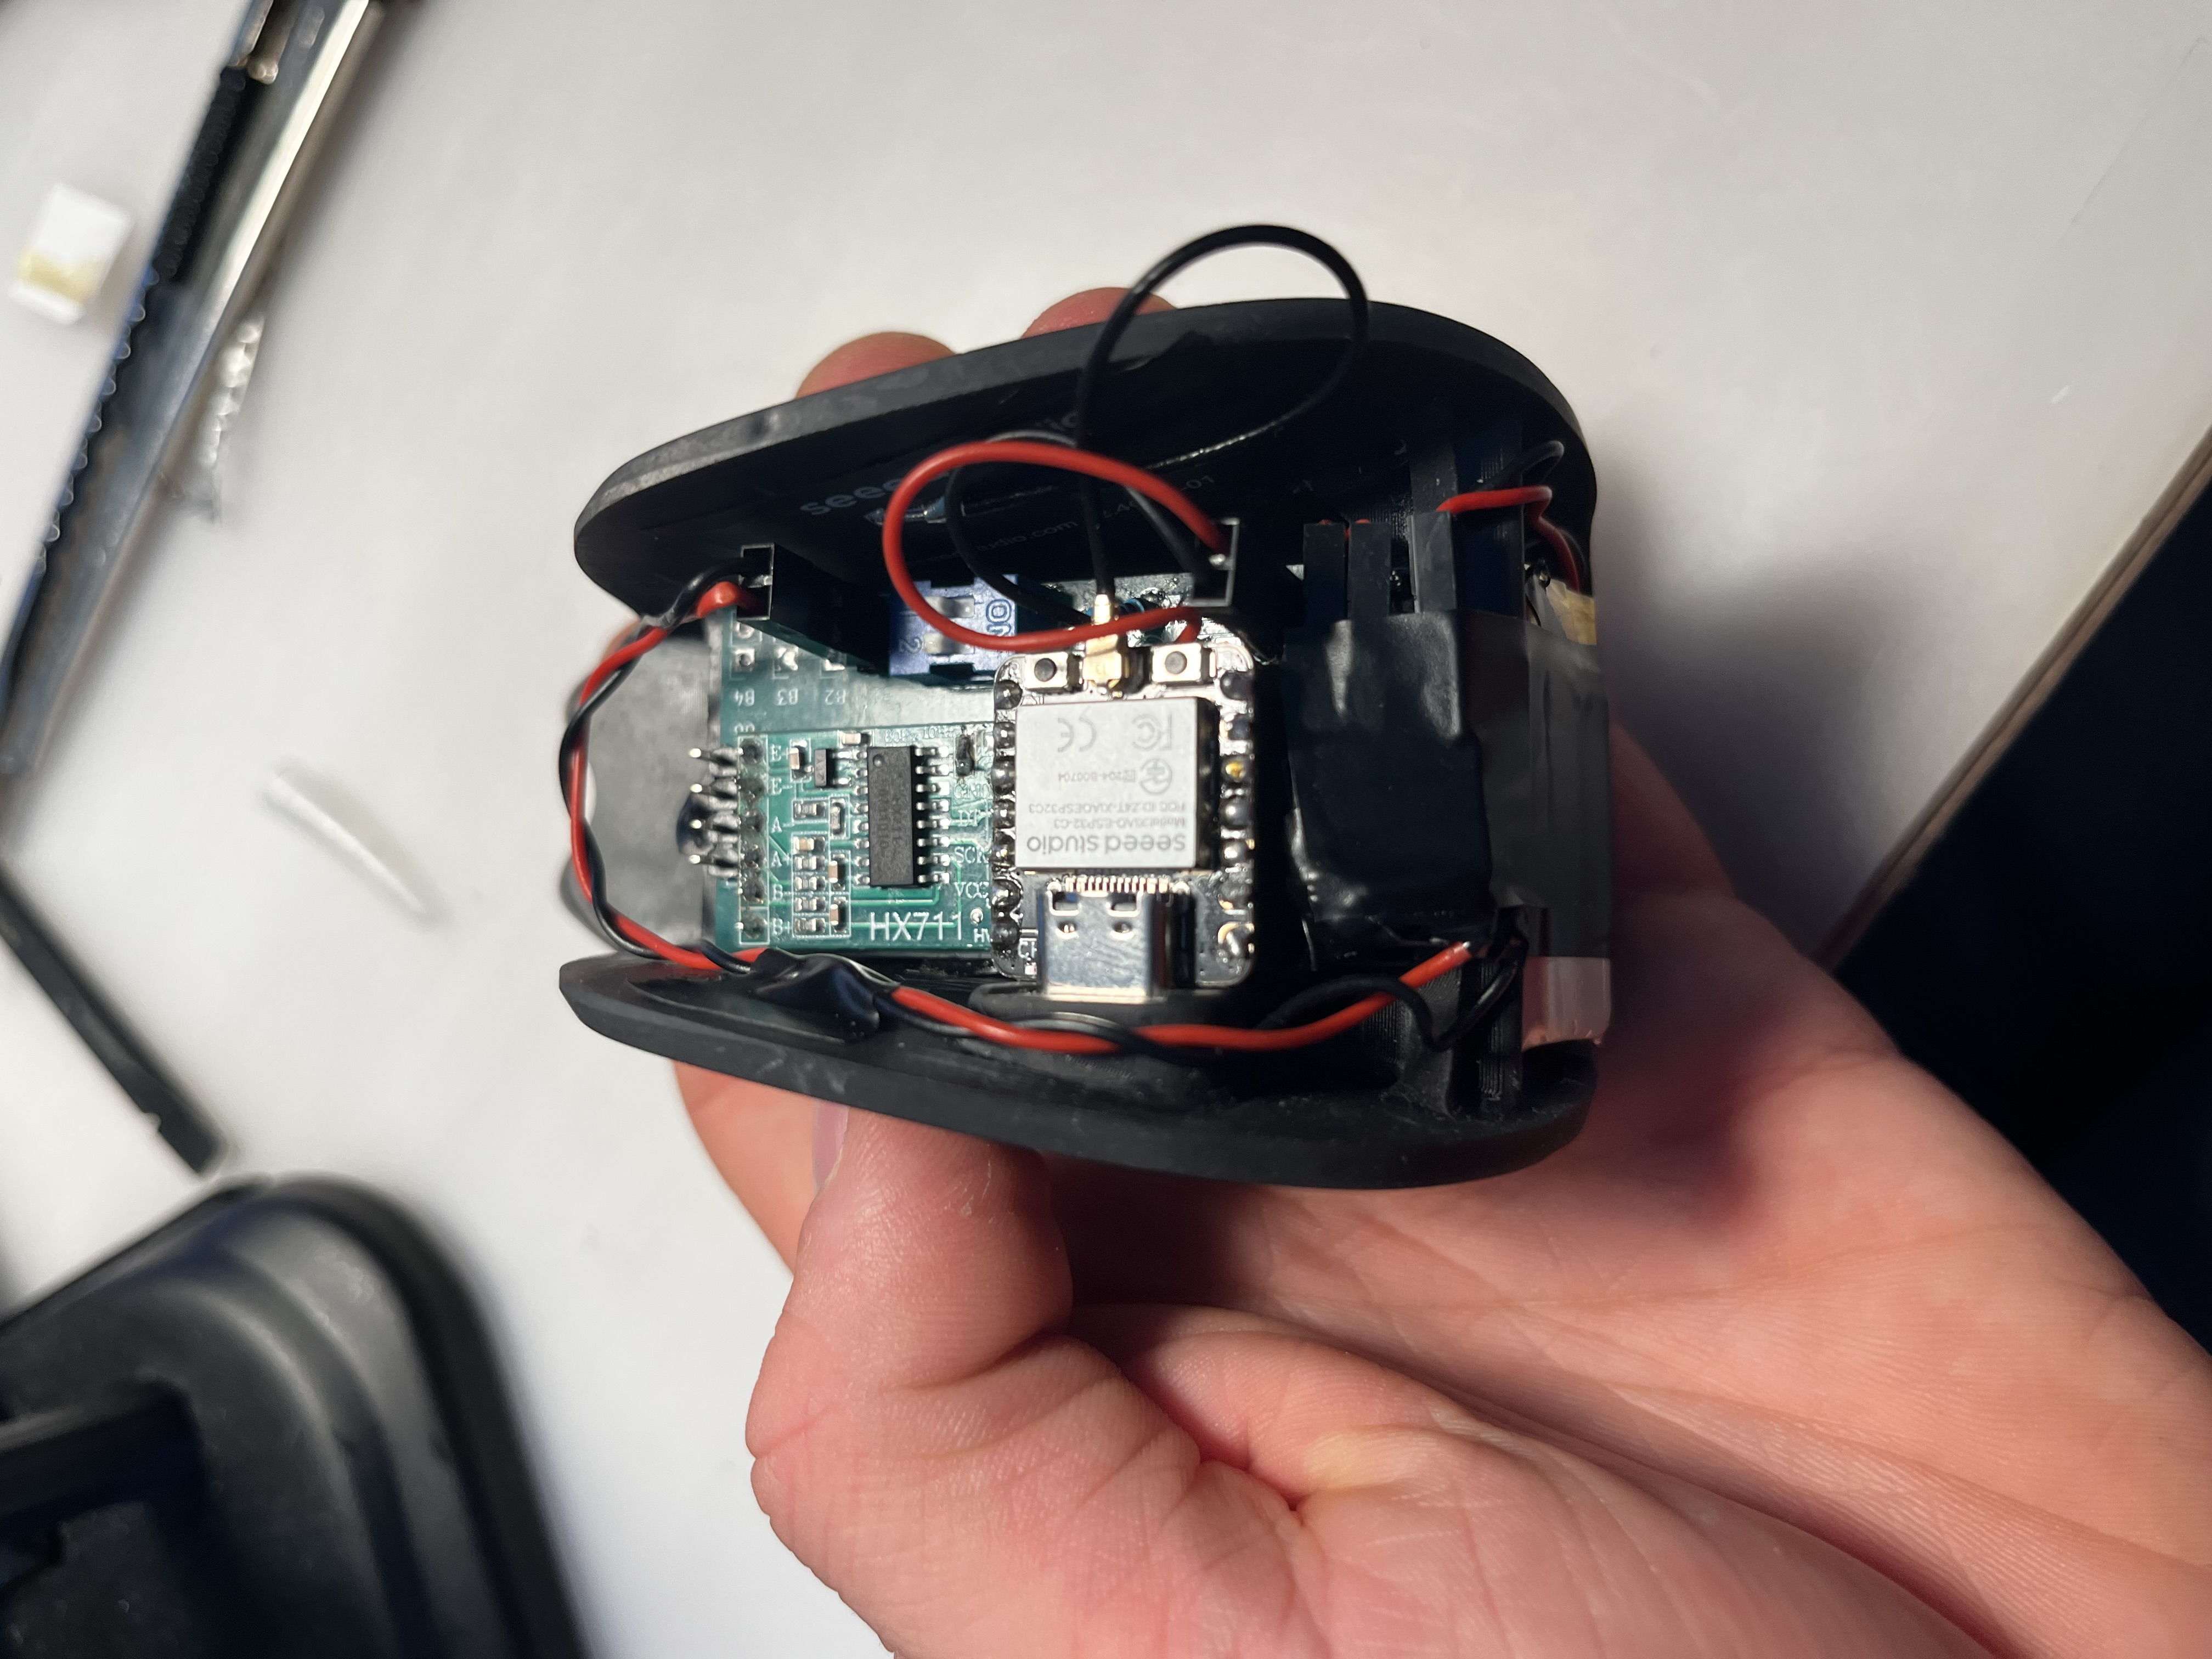
\includegraphics[width=\linewidth]{05_figures/06_preliminary/prototype_interior}
    \caption{Interior of the prosthetic housing showing the custom PCB with
             the XIAO ESP32-C3 (centre), HX711 ADC (bottom), and wiring.}
    \label{fig:prototype_interior}
  \end{minipage}
\end{figure}

\begin{table}[h]
  \centering
  \caption{Main hardware components of the prototype.}
  \label{tab:hw_components}
  \begin{tabular}{llll}
    \toprule
    \textbf{Component} & \textbf{Model} & \textbf{Interface} & \textbf{Role} \\
    \midrule
    Microcontroller     & XIAO ESP32-C3        & ---    & Processing, storage, communication \\
    IMU                 & MPU-9250 + AK8963    & SPI    & Accel, gyroscope, magnetometer \\
    Load cell ADC       & HX711                & 2-wire & Force digitisation (24-bit) \\
    Force sensor        & LCR02                & Analog & Inline axial force measurement \\
    Storage             & MicroSD (SPI module) & SPI    & Local data storage \\
    Battery             & LiPo 250\,mAh × 2   & ---    & 500\,mAh @ 3.7\,V \\
    \bottomrule
  \end{tabular}
\end{table}

% ----------------------------------------------------------------------
\section{Firmware and Data Pipeline}
\label{section:firmware}

The firmware runs on the Arduino/PlatformIO framework at a target rate of
80\,Hz (constrained by the HX711).
Each sample cycle reads force and all nine IMU axes, applies a first-order
low-pass filter to the force signal ($\alpha=0.2$), updates a
quaternion-based complementary filter for orientation estimation
($\alpha_\text{gyro}=0.97$), and appends the result to a CSV session file
on the SD card.

Each CSV row records: microsecond timestamp, wall-clock time (NTP-synced),
battery voltage, raw and calibrated force (kg), the nine IMU axes, and
estimated roll/pitch/yaw.
Sessions are stored under a hierarchical directory structure
(\texttt{/inbox/YYYYMMDD/}) with filenames encoding date, time, and run
number for unambiguous identification.

The system exposes a browser-accessible web interface (HTTP, port 80) with
real-time status (force, orientation, battery, sample count) updated via
WebSocket at 10\,Hz, as well as start/stop session controls and direct CSV
download.
Wi-Fi can be disabled at runtime to extend battery life during field
acquisition.

% ----------------------------------------------------------------------
\section{Sensor Validation}
\label{section:sensor_validation}

\subsection{System Boot and Peripheral Detection}

All peripherals initialised without errors on first power-up: the MPU-9250
reported \texttt{WHO\_AM\_I\,=\,0x73}, the AK8963 magnetometer reported
\texttt{WHO\_AM\_I\,=\,0x48}, and the HX711 and SD card also confirmed
successful initialisation.
Wi-Fi connected and NTP time synchronisation completed within 5\,s of boot.

\subsection{Load Cell Calibration}

The HX711 was calibrated by placing known reference weights on the load cell
and recording the corresponding raw ADC output.
The calibration factor $k = 18\,570$\,counts/kg was determined empirically
and applied in firmware:
\begin{equation}
  \hat{w} = \frac{r - r_0}{k}
  \label{eq:hx711_calib}
\end{equation}
where $r$ is the raw ADC reading and $r_0$ is the zero-load tare offset.
The calibration was verified by comparing the estimated weight against
reference loads across the expected operating range.

It should be noted that the current values of $r_0$ and $k$ are preliminary,
obtained under informal bench conditions using a small number of reference
points.
This single-point approach does not account for potential non-linearity,
temperature drift, or mechanical creep of the load cell, and is therefore
insufficient for rigorous cross-session quantitative comparison.
To address this limitation, a dedicated calibration rig is currently under
construction. The instrument will allow controlled and repeatable application
of certified reference loads across the full expected operating range,
enabling a robust multi-point calibration curve to be established prior to
the main data collection phase.
Figure~\ref{fig:calib_rig} shows the calibration rig under preparation.

\begin{figure}[ht]
  \centering
  % TODO: replace with actual photo
  % \includegraphics[width=0.75\linewidth]{05_figures/06_preliminary/calib_rig}
  \fbox{\rule{0pt}{6cm}\rule{0.75\linewidth}{0pt}}
  \caption{Calibration rig under construction for multi-point load cell
           characterisation across the full operating force range.}
  \label{fig:calib_rig}
\end{figure}

\subsection{Orientation Estimator}

The complementary filter was verified by placing the device in known static
orientations and confirming that the reported Euler angles (roll, pitch, yaw)
matched the expected values.
Dynamic tracking was assessed by moving the device through controlled
rotations; the filter converged within 1--2\,s of motion onset and tracked
attitude smoothly without observable drift over sessions of several minutes.

% ----------------------------------------------------------------------
\section{Preliminary Data Collection}
\label{section:preliminary_data}

\subsection{Data Collection Sessions}

An initial field session was conducted on 28 May 2026 with the prototype
fitted to a canine subject, comprising 11 acquisition runs following a
warm-up period.
This session confirmed correct system operation under real conditions and
provided a first dataset for signal characterisation.
Data collection was carried out in collaboration with the Hospital
Veterinário de Lisboa (São Bento), whose clinical team provided access to
real canine patients fitted with prosthetic devices and assisted with animal
handling during the acquisition sessions.
The physical construction of the instrumented prosthesis and the calibration
rig was supported by Composites Kingdom, who contributed materials expertise
and fabrication assistance.

Each run consists of a continuous recording at 80\,Hz, with individual
runs lasting between 30 and 180\,s.

\subsection{Signal Characteristics}

The acquired signals exhibit clear and reproducible characteristics consistent
with the expected biomechanics of locomotion.
The force channel shows distinct periodic peaks corresponding to ground
contact events, with a regular inter-peak interval reflecting stride duration.
The accelerometer vertical axis captures the characteristic profile of the
stance phase, while the roll and pitch channels reflect prosthesis orientation
dynamics during the gait cycle.

The periodic structure of gait is clearly visible in both the force and
inertial channels, confirming that the system captures the essential temporal
features of a locomotion cycle under real conditions.

Figure~\ref{fig:signal_overview} shows the force and vertical acceleration
signals recorded during a representative walking session, with the
characteristic periodic pattern of the gait cycle clearly present in
both channels.
Figure~\ref{fig:signal_imu} shows the orientation angles estimated by the
complementary filter during the same session.

The Euler angles are presented in \textit{unwrapped} form: instead of
resetting to the $[0°, 360°)$ range when a boundary is crossed, the
angle accumulates continuously (e.g.\ $359° \rightarrow 361° \rightarrow 362°$).
This eliminates the artificial discontinuities that would otherwise appear
as large instantaneous jumps in the plotted curves.
As a consequence, a complete $360°$ rotation by the animal results in a
net accumulated offset rather than a return to the initial value ---
which is the physically correct representation of total angular displacement.

\begin{figure}[ht]
  \centering
  \includegraphics[width=0.95\linewidth]{05_figures/06_preliminary/signal_overview}
  \caption{Force (top) and vertical acceleration $a_z$ (bottom) recorded
           during a canine walking session (run~9, 28 May 2026).
           The periodic structure of the gait cycle is clearly visible in
           both channels throughout the session, which includes a straight
           walking segment and a return pass after a turn.}
  \label{fig:signal_overview}
\end{figure}

\begin{figure}[ht]
  \centering
  \includegraphics[width=0.95\linewidth]{05_figures/06_preliminary/signal_imu}
  \caption{Vertical acceleration (top) and estimated roll, pitch and yaw
           angles (bottom, yaw unwrapped) during the same canine walking
           session. The yaw trend reflects the directional change during
           the turn; roll and pitch capture the prosthesis tilt dynamics
           at stride frequency.}
  \label{fig:signal_imu}
\end{figure}

\subsection{Data Quality and Firmware Correction}

Post-processing of the acquired runs identified a firmware bug present in an
earlier software version: a redundant blocking read caused the force estimate
to freeze for up to 20 consecutive samples, and a timeout path produced
spurious raw ADC values near 2\,500 counts.
Both issues have been corrected in the current firmware.
The affected sessions were cleaned using a post-processing script that removes
spurious samples (approximately 21\% of the raw total) and recomputes the
force estimate per sample from the raw ADC value using
Equation~\ref{eq:hx711_calib}.
The corrected dataset forms the basis for subsequent feature extraction and
model development.

% ----------------------------------------------------------------------
\clearpage
\section{Current Limitations}
\label{section:current_limitations}

The current prototype presents several limitations to be addressed in
subsequent phases.

\textbf{Dataset.}
The preliminary dataset consists of a single informal field session.
Structured acquisition campaigns with multiple canine subjects and sessions
are required to build a dataset suitable for model training and validation.

\textbf{IMU mounting calibration.}
The sensor is mounted in an arbitrary orientation within the prosthetic
housing.
A rotation matrix aligning the sensor frame with the prosthetic anatomical
frame has been derived, but integration into the main firmware is pending.

\textbf{Power autonomy.}
Estimated autonomy figures are based on measured current draw; validation
through a full discharge cycle is planned.

\textbf{Load cell calibration range.}
A formal multi-point calibration against certified weights across the full
expected force range is planned before quantitative cross-session comparison.
